%
% teil1.tex -- Beispiel-File für das Paper
%
% (c) 2020 Prof Dr Andreas Müller, Hochschule Rapperswil
%
%
% teil2.tex -- Beispiel-File für teil2 
%
% (c) 2020 Prof Dr Andreas Müller, Hochschule Rapperswil
%%



\rhead{Kalman-Filter}

\section{Kalman-Filter}
Da wir die äussere Kraft nicht direkt messen können, benötigen wir ein Werkzeug, welches aus der gemessenen Position, die Krafteinwirkung auf unsere System schätzt. 
Dies ist eine Typische Anwendung für den linearen Kalman-Filter.
Unser Ziel ist es, anhand der Messung die eigentlich interessante Grösse $f$ zu bestimmen. 
Dabei wird durch eine deterministische Vorhersage, in dem der Zustand * Eigendynamik des Systems gerechnet. 
Die Idee dahinter ist, dass das Kalman-Filter die nicht-deterministische Grösse $f$ anhand der Messung und der Vorhersage zu bestimmen.

Für mehrere Dimensionen (x,y,z) würde der Pythagoras für das System benötigt werden.
Da sich der Pythagoras bekanntlich nicht linear verhält, kann kein lineares Kalman-Filter implementiert werden. 
Da das Kalman-Filter besonders effektiv und einfach für lineare Abläufe geeignet ist, würde eine zweidimensionale Betrachtung den Rahmen dieser Arbeit sprengen. 
Für ein nicht-lineares System werden Extended Kalman-Filter benötigt, bei denen die System-Matrix (A) durch die Jacobi-Matrix des System ersetzt wird.
Einfachheitshalber beschränken wir uns auf den linearen Fall, da dadurch die wesentlichen Punkte bereits aufgezeigt werden. 

\subsection{Geschichte}
Das Kalman-Filter wurde 1960 von Rudolf Emil Kalman entdeckt und direkt von der NASA für die Appollo Mission benutzt. Der Filter kommt mit wenig Rechenleistung aus und war somit dafür geeignet die Rakete bei der Navigation zu unterstützen. Das Filter schätzt den Zustand eines Systems anhand von Messungen und kann den nächsten Zustand errechnen. Eine typische Anwendungen des Kalman-Filters ist Glättung von verrauschten Daten und die Schätzung von Parametern. Dies kommt heutzutage in jedem Satellit, Navigationssystem, Smartphones und Videospielen vor.

\subsection{Wahrscheinlichkeit}
Das Kalman-Filter schätzt den wahrscheinlichsten Wert zwischen Normalverteilungen.
Dies bedeutet, das Filter schätzt nicht nur den Mittelwert, sondern auch die Standartabweichung.
Da Normalverteilungen dadurch vollständig definiert sind, schätzt ein Kalman-Filter die gesamte Verteilungsfunktion des Zustandes.
Die eine Funktion zeigt die errechnete Vorhersage des Zustands, bzw. deren Normalverteilung. 
Die andere Funktion zeigt die verrauschte Messung des nächsten Zustand, bzw. deren Normalverteilung. 
Wie man am Beispiel der Gauss-Verteilungen unten sehen kann, ist sowohl der geschätzte Zustand als auch der gemessene Zustand normalverteilt und haben dementsprechend unterschiedliche Standardabweichungen $\sigma$ und Erwartungswerte $\mu$.

\begin{figure}
 \begin{center}
 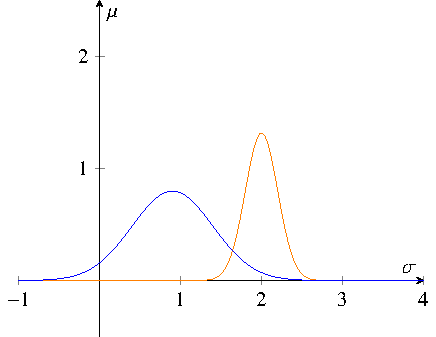
\includegraphics[width=5cm]{papers/erdbeben/Gausskurve2.pdf}
 \caption{Zwei Normalerteilungen; Die eine Funktion zeigt die Vorhersage, die andere die Messung}
 \end{center}
\end{figure}


Um eine genauere Schätzung des Zustandes zu machen, wird nun ein Wert zwischen den beiden Verteilungen berechnet. 
Nun wird eine Eigenschaft der Normalverteilung ausgenutzt. Durch das Multiplizieren zweier Normalverteilungen entsteht eine neue Normalverteilung. 
Wir haben eine Normalverteilung der Vorhersage:

\[ {y_1}(x;{\mu_1},{\sigma_1})=\frac{1}{\sqrt{2\pi\sigma_1^2}}\quad e^{-\frac{(x-{\mu_1})^2}{2{\sigma_1}^2}} \]
und der Messung:
\[ {y_2}(x;{\mu_2},{\sigma_2})=\frac{1}{\sqrt{2\pi\sigma_2^2}}\quad e^{-\frac{(x-{\mu_2})^2}{2{\sigma_2}^2}}. \]



Diesen werden nun Multipliziert und durch deren Fläche geteilt um sie wieder zu Normieren:
\[
{y_f}(x;{\mu_f},{\sigma_f})=\frac{ \frac{1}{\sqrt{2\pi\sigma_1^2}}e^{-\frac{(x-{\mu_1})^2}{2{\sigma_1}^2}} \cdot \frac{1}{\sqrt{2\pi\sigma_2^2}}e^{-\frac{(x-{\mu_2})^2}{2{\sigma_2}^2}}}{\int {y_1}\cdot{y_2} dx\,}
 \] 

Diese Kombination der beiden Verteilungen resultiert wiederum in einer Normalverteilung
\[ {y_f}(x; {\mu_f}, {\sigma_f}) = {y_1}(x;{ \mu_1},{ \sigma_1}) {\cdot y_2}(x; {\mu_2}, {\sigma_2}), \]
mit Erwartungswert
\[ \mu_f = \frac{\mu_1\sigma_2^2 + \mu_2 \sigma_1^2}{\sigma_1^2 + \sigma_2^2} \]
und Varianz
\[ \sigma_f^2 = \frac{\sigma_1^2 \sigma_2^2}{\sigma_1^2 + \sigma_2^2}. \]

Dadurch gleicht sich die neue Kurve den anderen an. Interessant daran ist, dass die fusionierte Kurve sich der genauere Normal-Verteilung anpasst.
Ist ${\sigma_2}$ klein und ${\sigma_1}$ gross, so wird sich die fusionierte Kurve näher an ${y_2}(x;{\mu_2},{\sigma_2})$ begeben.
Sie ist also gewichtet und die best mögliche Schätzung. 


\begin{figure}
 \begin{center}
 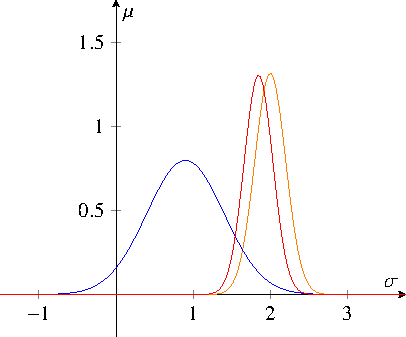
\includegraphics[width=5cm]{papers/erdbeben/Gausskurve3.pdf}
 \caption{Durch das Multiplizieren der blauen und der orangen Verteilung entsteht die die rote, optimale Funktion}
 \end{center}
\end{figure}


Was in 2 Dimensionen erklärt wurde, funktioniert auch in mehreren Dimensionen. 
Dieses Prinzip mach sich das Kalman Filter zu nutze, und wird von uns für die Erdbeben Berechnung genutzt. 

\section{Filter-Matrizen}
Um den Kalman Filter zu starten, müssen gewisse Bedingungen definiert werden. 
In diesem Abschnitt werden die einzelnen Parameter und Matrizen erklärt und erläutert, wofür sie nützlich sind. 

\subsection{Anfangsbedingungen}
\subsubsection*{Anfangszustand $x$}
Das Filter benötigt eine Anfangsbedingung. 
In unserem Fall ist es die Ruhelage, die Masse bewegt sich nicht. 
Zudem erfährt die Apparatur keine äussere Kraft.


\[ {x_0 }= \left( \begin{array}{c} {s_0}\\ {v_0}\\{f_0}\end{array}\right) = \left( \begin{array}{c} 0\\ 0\\ 0\end{array}\right) \]

\subsubsection*{Anfangsfehler / Kovarianzmatrix $P$}
Da auch der Anfangszustand fehlerhaft sein kann, wird für das Filter ein Anfangsfehler verwendet. 
Auf der Diagonalen werden die Varianzen eingesetzt, in den restlichen Felder stehen die Kovarianzen.
Zur Erinnerung: Die Varianz ist ein Mass für die Streuung eines Wertes, die Kovarianz hingegen beschreibt die Abhängigkeit der Streuungen zweier Werte.

Kovarianz: Cov(x, y) und Varianz: Var(x) = Cov(x, x)

In unserem Fall ist der Anfangszustand gut bekannt. 
Wir gehen davon aus, dass das System in Ruhe und in Abwesenheit eines Erdbeben startet, somit kann die Matrix mit Nullen bestückt werden. 
Als Initialwert für die für die Kovarianzmatrix ergibt sich

\[ 
{P_0 }=
\left(
\begin{array}{ccc} 	
0 & 0 &0 \\ 
0 &0 & 0 \\ 
0 & 0 &0 \\
\end{array}
\right).
 \] 
Diese Matrix beschreibt die Unsicherheit des geschätzten Zustandes und wird sowohl für die Vorhersage als auch die Korrektur benötigt. 
Sie wird nach jeder Schätzung aktualisiert. 
Für einen gut bekannten Zustandsvektor können kleine Werte eingesetzt werden, für ungenaue Anfangsbedingungen sollten grosse Werte verwendet werden. 
Grosse Werte ermöglichen dem Filter sich schnell einzupendeln. 

\subsubsection*{Dynamikmatrix $A$}
Das Kalman-Filter benötigt für die Vorhersage des nächsten Zustandes eine Beschreibung der Systemdynamik.
Die Dynamikmatrix bildet den Kern des Filters. Diese wurde weiter oben bereits beschrieben. 
Dabei wollen wird die äussere Kraft des Systems ermitteln.
Da nichts über die äussere Kraft bekannt ist, müssen wir annehmen das deren Ableitung 0 ist. 
Die System Vektor-Gleichung lautet daher:
\[ 
A = \left(
 \begin{array}{ccc} 	
0 & 1& 0 \\
- \frac{D}{m} &-\frac{2k}{m} & \frac{1} {m}\\
0 & 0& 0\\ 
\end{array}\right)  
 \]
Dabei soll der Kalman-Filter in diskreten Zeitschritten $\Delta t$ arbeiten. 
Die Übergangs-Matrix erhalten wir aus der Systemdynamikmatrix mittels Exponentialfunktion: 
\[\Phi = \exp(A\Delta t). \]

\subsubsection*{Prozessrauschkovarianzmatrix $Q$}
Die Prozessrauschmatrix teilt dem Filter mit, wie sich der Prozess verändert. 
Kalman-Filter berücksichtigen Unsicherheiten wie Messfehler und -rauschen. 
Bei unserem Modell könnte das beispielsweise ein Windstoss an die Masse sein. 
Für uns wäre dies:
\[ 
Q = \left(
 \begin{array}{ccc} 	
{\sigma_s }^2& 0& 0 \\ 
0 & {\sigma_v }^2& 0\\ 
0 & 0& {\sigma_f }^2\\
\end{array}\right)  
 \]

Die Standabweichungen müssten statistisch ermittelt werden, da der Fehler nicht vom Sensor kommt und somit nicht vom Hersteller gegeben ist. 
Das Bedeutet wiederum dass $Q$ die Unsicherheit des Prozesses beschreibt und nicht die der Messung.

\subsubsection*{Messmatrix $H$}
Die Messmatrix gibt an, welche Parameter gemessen werden
In unserem Falle ist es die Position der Massen. 

\[ H = (1, 0, 0) \]

\subsubsection*{Messrauschkovarianz $R$}
Die Messrauschkovarianzmatrix beinhaltet, wie der Name es schon sagt, das Rauschen der Positionsmessung. 
In unserem Fall wird nur die Position der Masse gemessen. Da wir keine anderen Sensoren haben ist $R$ lediglich:
\[ R= ({\sigma_{sensor}}^2).
 \] 
Diese Messrauchen wird meistens vom Sensorhersteller angegeben. 
Für unsere Theoretische Apparatur wird hier ein kleiner Fehler eingesetzt da heutige Sensoren sehr genau messen können. 

\subsection{Fiter-Agorithmus}
Nachdem alle Parameter aufgestellt sind, wird das Filter initialisiert.
Zuerst wird der nächste Zustand der Feder vorhergesagt, danach wird die Messung präzisiert und laufend zu aktualisieren. 
Das Filter berechnet aufgrund der aktuellen Schätzung eine Vorhersage. 
Diese wird, sobald verfügbar, mit der Messung verglichen. 
Aus dieser Differenz und den Unsicherheiten des Prozesses ($Q$) und der Messung ($R$) wird der wahrscheinlichste, neue Zustand geschätzt.

\subsubsection*{Vorhersage}
Im Filterschritt Vorhersage wird der nächste Zustand anhand des Anfangszustand und der Systemmatrix berechnet. 
Dies funktioniert mit dem Rechenschritt:
\[ 
{x_{k|k-1}}=\Phi \cdot {x_{k-1|k-1}}= \exp(A\Delta t)\cdot{x_{k|k-1}}.
 \] 

Die Kovarianz $P_{pred}$ wird ebenfalls neu berechnet. Da wir ein mehrdimensionales System haben, kommt noch die Prozessunsicherheit $Q$ dazu, so dass die Unsicherheit des Anfangsfehlers $P$ laufend verändert. 
Dies funktioniert durch multiplizieren der Systemmatrix mit dem aktualisierten Anfangsfehler. 
Dazu wird noch die Prozessunsicherheit addiert, somit entsteht die Gleichung
\[ {P_{k|k-1}} = {\Phi_k}  {P_{k-1|k-1}} {\Phi_k} ^T + {Q_{k-1}} .\] 
Es vergeht genau $dt$ Zeit, und dieser Vorgang wird wiederholt. 
Dabei wird in den späteren Schritten überprüft, wie genau die letzte Anpassung von $P$ zur Messung stimmt. 
Ist der Unterschied klein, wird die Kovarianz $P$ kleiner, ist der Unterschied gross, wird auch die Kovarianz grösser. 
Das Filter passt sich selber an und korrigiert sich bei grosser Abweichung.

\subsubsection*{Messen}
Der Sensor wurde noch nicht benutz, doch genau der liefert Werte für das Filter. 
Die aktuellen Messwerte $z$ werden die Innovation $w$ mit dem Zustandsvektor $x$ und der Messmatrix $H$ zusammengerechnet.
Hier bei wird lediglich die Messung mit dem Fehler behaftet, und die Messmatrix $H$ mit der Vorhersage multipliziert

\[{w_{k}}={z_{k}}-{H_{k}}\cdot{x_{k|k-1}}.\] 

Die Innovation ist der Teil der Messung, die nicht durch die Systemdynamik erklärt werden kann. 
Die Hilfsgröße Innovation beschreibt, wie genau die Vorhersage den aktuellen Messwert mittels der Systemmatrix $\phi$ beschreiben kann. 
Für eine schlechte Vorhersage wird die dazugehörige Innovation gross, für eine genaue Vorhersage dagegen klein sein. 
Entsprechende Korrekturen müssen dann gross bzw. nur gering ausfallen. 
Innovation = Messung - Vorhersage. Dies ist intuitiv logisch, eine Innovation von 0 bedeutet, dass die Messung nichts Neues hervorbrachte.

Im nächsten Schritt wir analysiert, mit welcher Kovarianz weiter gerechnet wird. 
Hierbei wird die Unsicherheit $P$, die Messmatrix $H$ und die Messunsicherheit $R$ miteinander verrechnet. 
\[ 
{S_{k}}={H_{k}}{P_{k|k-1}}{H_{k}}^T+{R_{k}}
 \] 

\subsubsection*{Aktualisieren}
Im nächsten Schritt kommt nun die Wahrscheinlichkeit nach Gauss dazu. 
\[ 
{K_{k}}= {{P_{k|k-1}} \cdot {H_{k}^T}}\cdot {S_{k}}^{-1} 
 \] 
Dieser Vorgang wird Kalman-Gain genannt. 
Er sagt aus, welcher Kurve mehr Vertraut werden soll, dem Messwert oder der Systemdynamik.
Das Kalman-Gain wird geringer wen der Messwert dem vorhergesagten Systemzustand entspricht. 
Sind die Messwerte komplett anders als die Vorhersage, wo werden die Elemente in der Matrix $K$ grösser.
Anhand der Informationen aus dem Kalman-Gain $K$ wird das System geupdated.

\[ 
{x_{k|k}}={x_{k|k-1}}+({K_{k}}\cdot {w_{k}}) 
 \] 

Dazu kommt  eine neue Kovarianz für den nächste Vorhersageschritt:

\[ 
{P_{k|k}}=(I-({K_{k}} \cdot {H_{k}})) \cdot {P_{k|k-1}}  
 \] 

Der ganze Ablauf wird nun zum Algorithmus und beginnt wieder mit der Vorhersage 

\[ 
{x_{k|k-1}}=\Phi \cdot {x_{k-1|k-1}}= \exp(A\Delta t)\cdot{x_{k|k-1}}.
 \] 


\subsection{Zusammenfassung }
Zusammenfassend kann das Kalman-Filter in offizieller Typus dargestellt werden. 
Dabei beginnt das Filter mit dem Anfangszustand für $k=0$

1. Nächster Zustand vorhersagen
\[{x_{k|k-1}}=\Phi \cdot {x_{k-1|k-1}}= \exp(A\Delta t)\cdot{x_{k|k-1}}.\] 

2. Nächste Fehlerkovarianz vorhersagen
\[{P_{k|k-1}}={\Phi _{k}} {P_{k-1|k-1}} {\Phi _{k}}^T + {Q_{k-1}}.\] 

3. Das Kalman Filter anwenden
\[{K_{k}}= {P_{k|k-1}} \cdot {H_{k}^T}\cdot {S_{k}^{-1}}\] 

4. Schätzung aktualisieren
\[{x_{k|k}}={x_{k|k-1}}+({K_{k}}\cdot {w_{k}}) \] 

5. Fehlerkovarianz aktualisieren
\[{P_{k|k}}=(I-({K_{k}}\cdot {H_{k}})) \cdot {P_{k|k-1}} \] 


6. Die Outputs von $k$ werden die Inputs für ${k-1}$ und werden wieder im Schritt 1 verwendet

